% !TEX root = PREN2_Dokumentation.tex
\section{System-Spezifikation}\label{SystemSpezifikation}
\subsection{Systemübersicht}
\subsubsection{Systemarchitektur}
\begin{figure}[H]
    \centering
    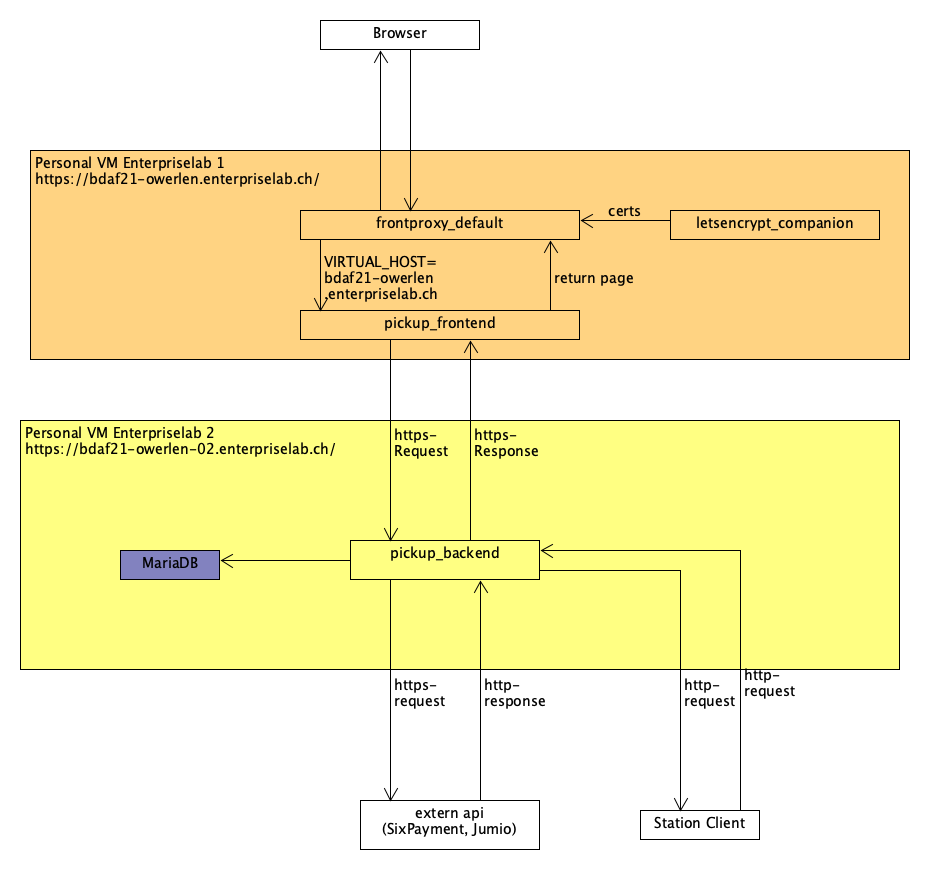
\includegraphics[width=1\textwidth]{images/system.png}
    \caption[Systemarchitektur]{Systemarchitektur, Quelle: Autor}
    \label{img: Systemarchitektur des Projektes}
\end{figure}
\newpage
\subsubsection{Kontextdiagramm}\label{Kontextdiagram}
\begin{figure}[H]
    \centering
   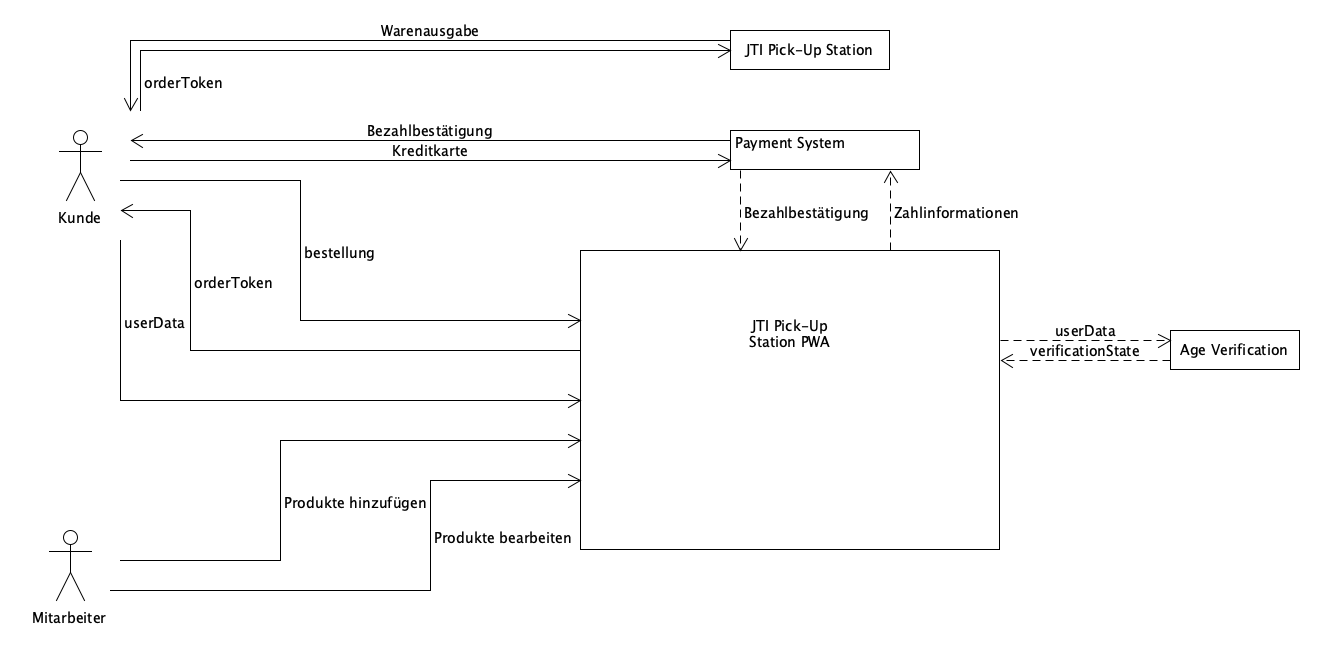
\includegraphics[width=1\textwidth]{images/kontextdiagramm.png}
    \caption[Kontextdiagramm]{Kontextdiagramm, Quelle: Autor}
    \label{img: Kontextdiagramm des Projektes}
\end{figure}
\newpage
\newpage
\subsection{Architektur und Designentscheide}
\subsubsection{Modelle und Sichten}
In diesem Projekt wird zwischen drei verschiedenen Sichten unterschieden:
\begin{itemize}
    \item \textbf{Kunde} Es handelt sich dabei um die Person, welche in der \ac{PWA} Produkte bestellt und diese abholt. 
    \item \textbf{Administrator} Dem Administrator ist es möglich, Produkt hinzuzufügen, zu verändern oder auch zu löschen. Er kann die kritischen Bestände an den Stationen abfragen. 
    \item \textbf{Programmierer} Dieser konzipiert und realisiert die Applikation gemäss den Anforderungen des Auftraggebers.
\end{itemize}
\newpage
\subsubsection{Daten (Mengengerüst und Strukturen)}
\paragraph{Datenbankschema}
Das Datenbankschema wurde von Intelij generiert. 
\begin{figure}[H]
    \centering
    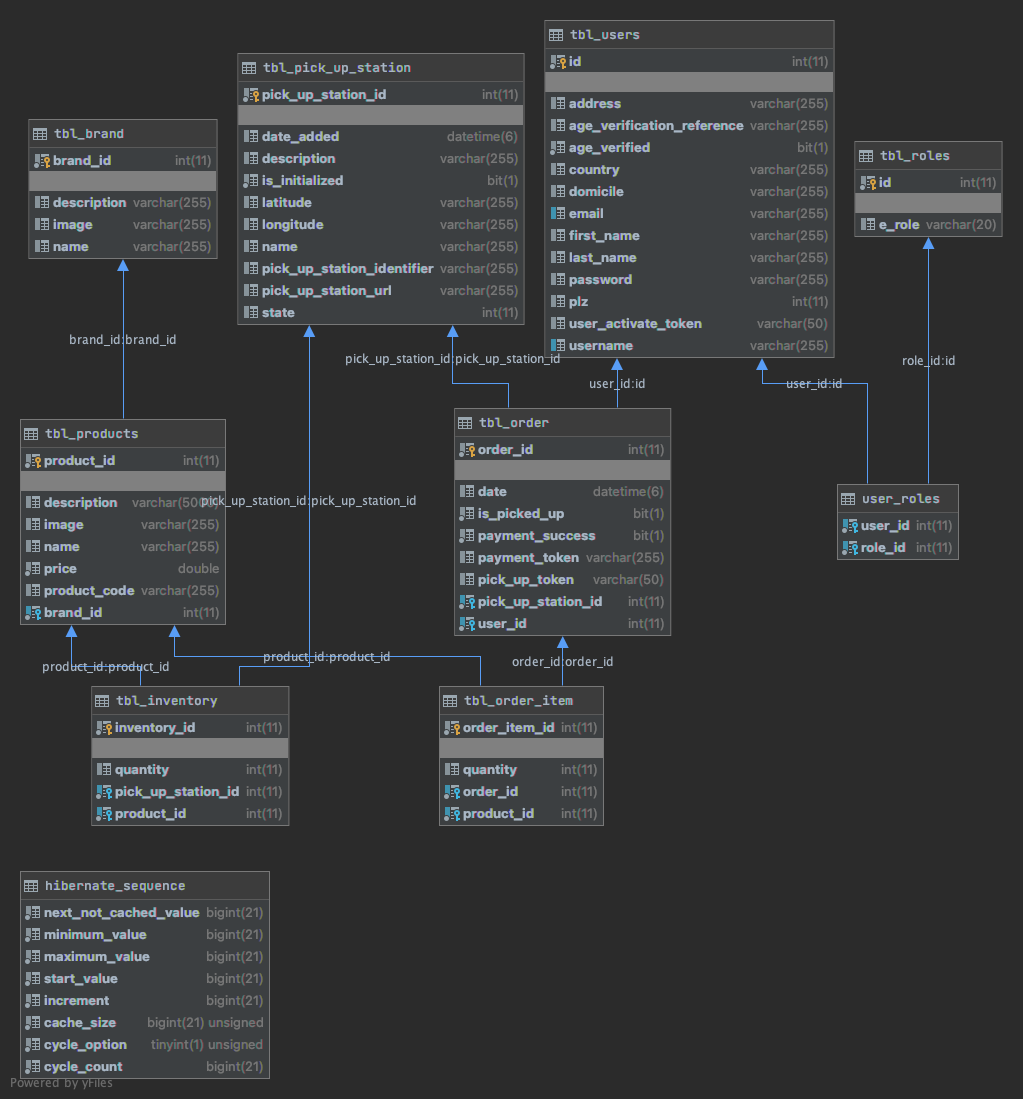
\includegraphics[width=1\textwidth]{images/databaseSchema.png}
    \caption[Datenbankschema]{Datenbankschema, Quelle: Autor}
    \label{img: datebankschema}
\end{figure}
\subsubsection{Entwurfsentscheide}
\paragraph{Frontend}
\subparagraph{Technologien}
\begin{itemize}
	\item Spring Boot 2.4.3
	\item Java 11
\end{itemize}
\subparagraph{Projektstruktur}
Im Projekt wurde eine einheitliche Projektstruktur verfolgt. Jeder Component befindet sich, zusammen mit den entsprechenden Services, in einem Ordner. Services ohne Component befinden sich in \glqq services\grqq{}. 
\subparagraph{Konfigurationen}
 Es wird zwischen produktiver und Entwicklungsumgebung unterschieden. Es wird nur die produktive Konfiguration aufgezeigt. 
\begin{verbatim}
	export const environment = {
		production: true, 
		appVersion: require('../../package.json').version,
		serverUrl: "https://bdaf21-owerlen-02.enterpriselab.ch:8080/api/v1/",
		paymentSucessfullRedirect: 
		"https://bdaf21-owerlen.enterpriselab.ch/checkPaymentAssert", 
		paymentNotSucessfullRedirect: 
		"https://bdaf21-owerlen.enterpriselab.ch/paymentError", 
		imageFolder: "assets/min/"
	};
	
\end{verbatim}
\paragraph{Backend}
\subparagraph{Technologien}
\begin{itemize}
	\item Spring Boot 2.4.3
	\item Java 11
\end{itemize}
\subparagraph{Projektstruktur}
Das Projekt ist in mehrere Packages aufgeteilt. 
\begin{itemize}
	\item Controller
	\item Services
	\item DTO
	\item Entities
	\item Repositories
\end{itemize}
\subparagraph{Data Transfer Object}\label{DTO}
Es handelt sich hier um ein Enterprise Application Architecture Pattern von Martin Fowler. Genauer handelt es sich um ein Distribution Pattern. \\
Durch den Einsatz dieses Patterns können mehr Daten mit einem Aufruf übertragen werden. Ein weiterer Vorteil ist die klare Trennung zwischen zu serialisierendem Objekt und dem Domain Model. In der Regel wird ein Assembler genutzt, um das DTO auf das Domain Model zu mappen. [\cite{dtoFowler}]
\begin{figure}[H]
	\centering
	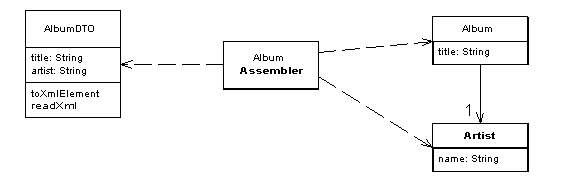
\includegraphics[width=1\textwidth]{images/dtoSketch.png}
	\caption[DTO Klassendiagramm von Martin Fowler]{DTO Klassendiagramm von Martin Fowler, Quelle: \cite{dtoFowler}}
	\label{img: dtoFowler}
\end{figure}
\subparagraph{\ac{HATEOAS}}
In diesem Projekt stand der Einsatz des DTO-Pattern jedoch im Konflikt mit der REST-Abstufung von Leonard Richardson und dem von ihm entworfenen Richardson Maturity Model. Gemäss diesem sollen Daten von einem anderen Domain Model als Hyperlink zurückgegeben werden, um das höchste Level zu erreichen. Somit liefert jeder Aufruf nur das angeforderte Modell zurück. Das Data Transfer Object Pattern dient somit nur zur Abgrenzung zwischen dem zu sendenden Objekt und dem Domain Model. 
Dabei wurde auf REST-Level 3 hingearbeitet \ref{img: richardsonMaturity} und mit \ac{HATEOAS} gearbeitet. Dadurch kann das Backend weiter vom Frontend getrennt werden, da bei eine Anpassung der URL auf dem Server keinen Einfluss auf die Funktionalität des Clients hat. Zudem kann die Verständlichkeit der API verbessert und ein Erweitern vereinfacht werden[\cite{richardsonMaturity}]. 
\subparagraph{Datenbank}
Die Datenbank wird durch die Spring Data JPA aus den Entities in diesem Projekt erstellt. 
\subparagraph{Konfigurationen}
Im Backend wurden die Konfigurationen im \gls{Propertie-File} vorgenommen. Es wird zwischen produktiver und Entwicklungsumgebung unterschieden. Vertrauliche Daten wurden bei der Dokumentation entfernt
\begin{verbatim}
	image.path=/var/
	spring.hateoas.use-hal-as-default-json-media-type=false
	
	# App Properties
	pickupbackend.app.jwtSecret= ""
	pickupbackend.app.jwtExpirationMs= 3600000
	pickupbackend.app.saferpay = ""
	
	#saferpay
	pickupbackend.app.saferpay.customerid = 257753
	pickupbackend.app.saferpay.terminalid = 17731797
	pickupbackend.app.saferpay.specVersion = 1.21
	
	#Jumio
	pickupbackend.app.jumio.username = ""
	pickupbackend.app.jumio.password = ""
	
	server.port= 8080
	security.require-ssl=false
	server.ssl.key-store=/etc/letsencrypt/live/
	bdaf21-owerlen-02.enterpriselab.ch/keystore.p12
	server.ssl.key-store-password = jtiPickUp2021
	server.ssl.keyStoreType= PKCS12
	server.ssl.keyAlias= tomcat
	
	springdoc.swagger-ui.path=/api/v1/swagger-ui/swagger-ui-custom.html
	
\end{verbatim}
\paragraph{Raspberry Pi Client}
\subparagraph{Technologien}
\begin{itemize}
	\item Node.js 14.14.0
	\item raspi-serial 6.0.0
	\item Raspberry Pi OS 
\end{itemize}
\subparagraph{Projektstruktur}
Bei diesem Projekt wurde die vorgegebene Projektstruktur von Node.js genutzt.

\subsection{Schnittstellen}
\subsubsection{Externe Schnittstellen}
\paragraph{REST API}
\subparagraph{API-Dokumention}
Die Spring Doc ermöglicht eine sehr einfache und schnelle Dokumentation von REST-API basierend auf der OpenAPI Spezifikation. Um die Dokumentation anzuzeigen, wird das Open Source Tool Swagger UI genutzt. Hiermit lässt sich eine dynamische API-Dokumentation als HTML-Page erstellen. 
\begin{figure}[H]
	\centering
	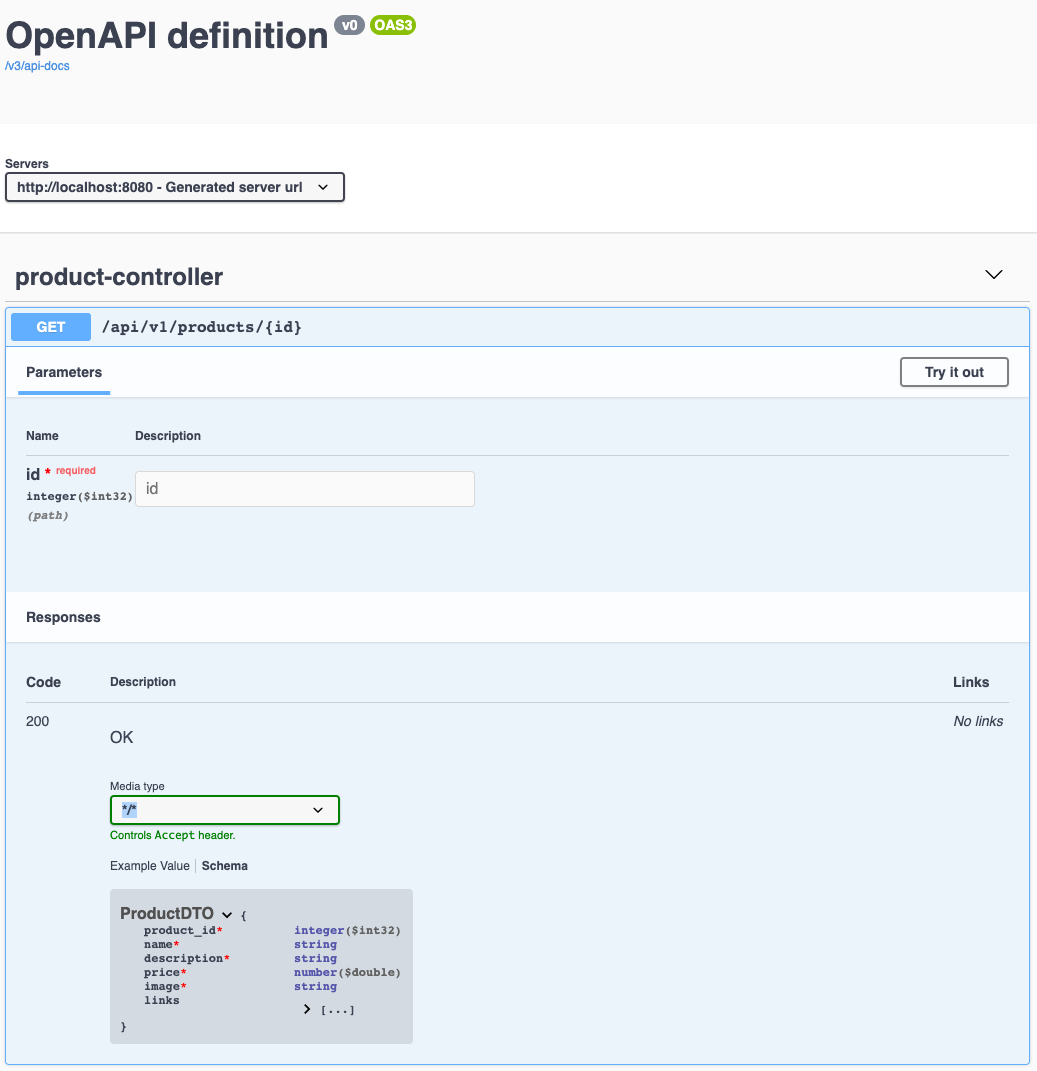
\includegraphics[scale=0.3]{images/swaggerui.png}
	\caption[Ausschnitt aus der Swagger Dokumentation]{Ausschnitt aus der Swagger Dokumentation, Quelle: Autor}
	\label{img: swaggerUI}
\end{figure}
\paragraph{Benutzerschnittstellen}
Auf ein Beschreiben der Benutzerschnittstelle wird an dieser Stelle verzichtet. 
\paragraph{Saferpay JSON-API}
Die \href{http://saferpay.github.io/jsonapi/}{JSON-API} von Six wird im offiziellen \gls{Github} Repository ausführlich beschrieben. 

\paragraph{Jumio API}
Die Jumio-API wird im \href{https://github.com/Jumio/implementation-guides}{Implementation Guide} beschrieben. 

\subsubsection{Wichtige interne Schnittstellen}
 \paragraph{UART-Übertragung}
 \subparagraph{Steckbrief}
Die Schnittstelle \ac{UART} wird für die Kommunikation zwischen Elektrotechnik und Informatik genutzt. 
\subparagraph{Interaktionen}
\begin{itemize}
	\item write
	\item read
\end{itemize}
 
 \subparagraph{Einsatz, Abläufe, Voraussetzungen und Zusicherung}
 \begin{itemize}
 	\item Um die Schnittstelle nutzen zu können, ist es nötig, am Serial Port \glqq serial0\grqq{} einen passenden Endpunkt angeschlossen zu haben.  
 	\item Das Node.js package \glqq raspi-serial\grqq{} muss installiert sein.
 \end{itemize}
 
 \subparagraph{Aufbau und Konfiguration}
 \begin{verbatim}
 	var serial = new Serial(DEFAULT_PORT = '/dev/serial0');
 \end{verbatim}
 \subparagraph{Fehlerbehandlung}
Eine explizite Fehlerbehandlung ist nicht vorhanden. 
 
 \subparagraph{Format}
 Die Daten müssen im folgenden Format übergeben werden: 
 \begin{verbatim}
 	productCode-productQuantity, 
 \end{verbatim}
 Es dürfen beliebig viele String kaskadiert werden. 
 \subparagraph{Beispielverwendung}
\begin{figure}[H]
	\centering
	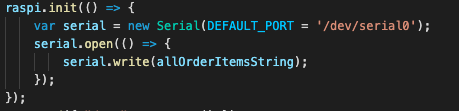
\includegraphics[scale=0.6]{images/sendDataUart.png}
	\caption[Senden von Daten via Schnittstelle]{senden von Daten via Schnittstelle, Quelle: Autor}
	\label{img: send}
\end{figure}

\begin{figure}[H]
	\centering
	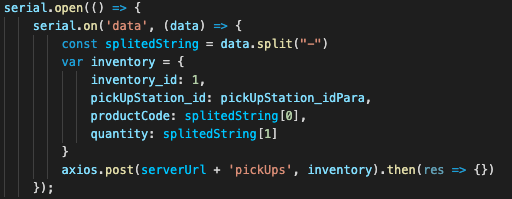
\includegraphics[scale=0.6]{images/readDataUart.png}
	\caption[Lesen von Daten via Schnittstelle]{Lesen von Daten via Schnittstelle, Quelle: Autor}
	\label{img: read}
\end{figure}

Eine weitere Beispielanwendung ist im Kapitel \ref{kommTiny} zu finden. 
\subsection{Environment-Anforderungen}\label{environmentanforderungen}
\subsubsection{Hardware}
Folgende Hardware wurde für diese Applikation verwendet und kann als ausreichend betrachtet werden:
\begin{itemize}
	\item CPU: Intel(R) Xeon(R) CPU E5-2630 v4 @ 2.20GHz
	\item RAM: 4GB
\end{itemize}
\subsubsection{Software}
Die ganze Applikation läuft auf virtuellen Maschine, auf der folgendes Betriebssystem installiert ist:
\begin{itemize}
	\item Ubuntu 20.04.01
	\item Docker 19.03.8
	\item certbot
\end{itemize}
\subsubsection{Kompatibilität}
\paragraph{Browser}
Die Software wurde auf den folgenden Browsern getestet. 
\begin{itemize}
	\item Safari 12
	\item Chrome 90
\end{itemize}
\newpage